\documentclass[aspectratio=169,nototalframenumber]{beamer}
\usetheme[nosectiontitlepage]{uibk}

\usepackage{tikz}
\usetikzlibrary{shapes}

\usepackage{pifont}
\newcommand{\done}{\textcolor{uibkblue}{\ding{52}}}
\newcommand{\unsure}{\textcolor{uibkorange}{?\,}}
\newcommand{\excluded}{\textcolor{red!88!black}{\ding{56}}}

\usepackage{graphicx}
\graphicspath{{fig/}}

\input{macros/mit-new.tex}
\usepackage{tikz}
\usetikzlibrary{arrows, patterns}

\RequirePackage{xcolor}
\definecolor{color1}{HTML}{7D0025}
\definecolor{color2}{HTML}{AB3816}
\definecolor{color3}{HTML}{C66D2E}
\definecolor{color4}{HTML}{DA9C5B}
\definecolor{color5}{HTML}{EAC486}
\definecolor{color6}{HTML}{F9E7AE}
\definecolor{color7}{HTML}{FFFFC8}

\newcommand{\legend}[2]{
  \begin{scope}[xshift=#1, yshift=#2]
    \draw[draw] (0,0) rectangle ++(3,-1);
    \draw[draw, fill=color1] (0.1,-0.1) rectangle ++(0.4,-0.2);
    \draw[anchor=west] (0.5, -0.2) node {\scriptsize Tensorflow time};
    \draw[draw, fill=color4] (0.1,-0.4) rectangle ++(0.4,-0.2);
    \draw[anchor=west] (0.5, -0.5) node {\scriptsize CPU time};
    \draw[draw, preaction={fill,color7}, pattern=north east lines] (0.1,-0.7) rectangle ++(0.4,-0.2);
    \draw[anchor=west] (0.5, -0.8) node {\scriptsize Enclave penalty};
  \end{scope}
}


\title{Enclave-NN}
\author{Alexander Schl\"ogl}

\begin{document}

\uibktitlepage{}

\begin{frame}[label=basics]
    \frametitle{Introduction}

    Neural Nets are universal approximators.

	\vspace{4ex}

	\begin{block}{Technical Details}
    	\begin{itemize}
        	\item Forward pass is a series of algebraic operations
        	\item Fully defined by their architecture and weights (parameters)
    	\end{itemize}
	\end{block}

	We focus solely on inference phase, so NNs for us are static functions.
\end{frame}

\begin{frame}
    \frametitle{Problem Statement}

	Monetization requires keeping parameters private.
	\vspace{3ex}
	\pause

	\begin{block}{Current Method}
    	Online Oracles
    	\begin{itemize}
        	\item parameters never public
        	\item require sharing of data for inference
        	\item require provider's infrastructure
    	\end{itemize}
	\end{block}

	\pause

	\begin{alertblock}{Idea}
    	Use Trusted Execution Environments (TEEs) to hide parameters during inference
	\end{alertblock}
\end{frame}

\begin{frame}
    \frametitle{Approach}

	\begin{figure}
    	\begin{tikzpicture}
        	\mitnetsummary{2}

			\onslide<2->{
    			\draw[draw=uibkgray,fill=uibkgray] (6,-.0) rectangle ++(.5,-.8);
    			\draw[draw=uibkgray,fill=uibkgray] (5.75,-.8) -- ++(1,0) -- ++(-.5,-.4) -- cycle;

            	\mitnetsummary{-2}
			}

			\onslide<2>{
				\draw[text=uibkblue!100,draw=uibkblue,fill=uibkblue!30,fill opacity=0.7,line width=0.5mm] (9.96,-1.6) coordinate (teebox) rectangle (12.5, -4);
                \draw node[text=uibkblue, anchor=north west] at (teebox) {\small TEE};
            }
			\onslide<3>{
				\draw[text=uibkblue!100,draw=uibkblue,fill=uibkblue!30,fill opacity=0.7,line width=0.5mm] (7.465,-1.6) coordinate (teebox) rectangle (12.5, -4);
                \draw node[text=uibkblue, anchor=north west] at (teebox) {\small TEE};
            }
			\onslide<4>{
				\draw[text=uibkblue!100,draw=uibkblue,fill=uibkblue!30,fill opacity=0.7,line width=0.5mm] (0.46,-1.6) coordinate (teebox) rectangle (12.5, -4);
                \draw node[text=uibkblue, anchor=north west] at (teebox) {\small TEE};
            }
		\end{tikzpicture}
	\end{figure}
\end{frame}

\begin{frame}
    \frametitle{Approach}

	Move last $n$ layers into TEE, send protected model to user
	\vfill
	\begin{minipage}{0.44\textwidth}
		\begin{block}{Advantages}
			Less infrastructure required\par
			Semi offline usage possible\par
			Inference data can stay private\par
		\end{block}
	\end{minipage}%
	\hfill%
	\begin{minipage}{0.44\textwidth}
		\begin{block}{Disadvantages}
			Performance impact\par
			Requires trust in manufacturer\par
			Potentially larger attack surface\par
		\end{block}
	\end{minipage}

\end{frame}

\begin{frame}
    \frametitle{Evaluation Method}
	How large is the performance impact?\par
	\begin{block}{Procedure}
	\begin{enumerate}
		\item Split NN
		\item Compile TEE and native code
		\item Measure inference time on single input
		\item Separate CPU impact from TEE impact
	\end{enumerate}
	\end{block}

	\vspace{1cm}
	Repeat for every possible split in NN
\end{frame}

\begin{frame}
    \frametitle{Results}

\begin{tikzpicture}[>=stealth,yscale=0.8]
  \draw (0,0) -- (\mitnetwidth,0);
  \foreach \x in \mitxticks {
    \draw (\x,0) -- (\x, -0.1);
  }

  \draw[->] (0,0) -- (0,\ymax+0.1);
  \foreach \y in \yticks {
    \draw (-0.1,\y) -- (0.1,\y);
  }
  \ylabels{-.5}
  
  \mitnetsummary{-0.2}

  \mitencryptedsplita
  \mitencryptedsplitb
  \mitencryptedsplitc
  \mitencryptedsplitd
  \mitencryptedsplite
  \mitencryptedsplitf
  \mitencryptedsplitg
  \mitencryptedsplith
  \mitencryptedspliti
  \mitencryptedsplitj
  \mitencryptedsplitba
  \mitencryptedsplitbb
  \mitencryptedsplitbc
  \mitencryptedsplitbd
  \mitencryptedsplitbe
  \mitencryptedsplitbf
  \mitencryptedsplitbg
  \mitencryptedsplitbh
  \mitencryptedsplitbi
  \mitencryptedsplitbj
  \mitencryptedsplitca
  \mitencryptedsplitcb
  \mitencryptedsplitcc
  \mitencryptedsplitcd
  \mitencryptedsplitce

  \legend{9cm}{6.3cm}

\end{tikzpicture}
\end{frame}

\begin{frame}
    \frametitle{Open Problem: Where to stop}

	\begin{itemize}
    	\item[\done] Generate weights
    	\item[\done] Generate code for forward pass
    	\item[\done] Interoparability with TF
    	\item[\done] Run forward pass in TEE
    	\item[\done] Hide weights
    	\item[\unsure] Hide architecture
    	\item[\unsure] Monetization prototype
    	\item[\unsure] Different TEE technologies
    	\item[\excluded] Automate for more code (TEE compiler target)
	\end{itemize}
\end{frame}

\begin{frame}
    \frametitle{Open Problem: Where to send it}

    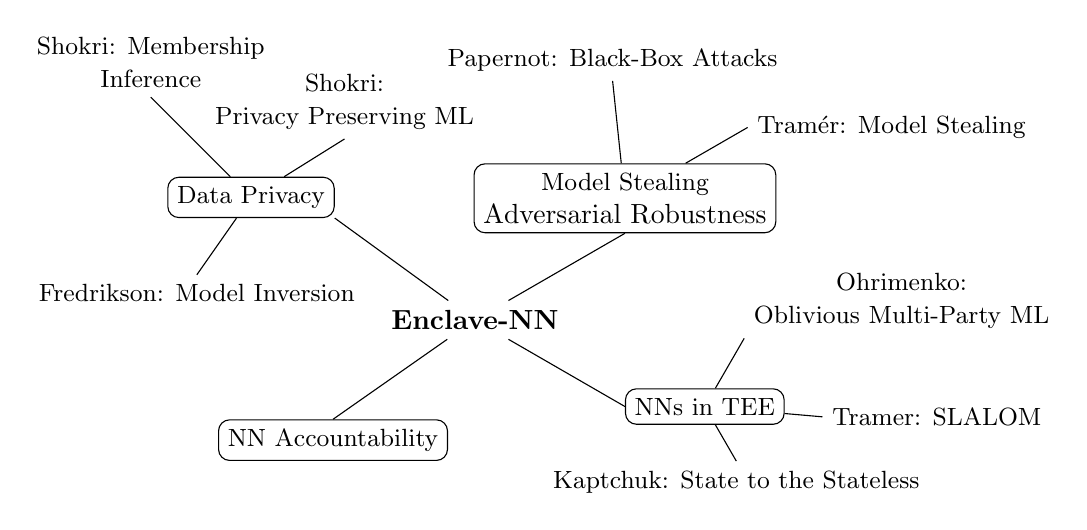
\begin{tikzpicture}
        \node at (0,0) (enclave-nn) {\textbf{Enclave-NN}};

        \draw (enclave-nn) -- (215:2.2) node[below,draw,rounded corners] (nn-accountability) {\small NN Accountability};

        \draw (enclave-nn) -- (30:2.2) node[above,align=center,draw,rounded corners] (model-stealing) {\small Model Stealing \\ Adversarial Robustness};
        \draw(model-stealing) -- ++(30:1.8) node[right] (stealing-tramer) {\small Tram\'er: Model Stealing};
        \draw(model-stealing) -- ++(96:1.5) node[above] (adv-papernot) {\small Papernot: Black-Box Attacks};

        \draw (enclave-nn) -- (-30:2.2) node[right,draw,rounded corners] (nn-enclave) {\small NNs in TEE};
        \draw (nn-enclave) -- ++(60:1) node[above right,align=center] {\small Ohrimenko:\\ \small Oblivious Multi-Party ML};
        \draw (nn-enclave) -- ++(300:0.8) node[below] {\small Kaptchuk: State to the Stateless};
        \draw (nn-enclave) -- ++(-5:1.5) node[right] {\small Tramer: SLALOM};

        \draw (enclave-nn) -- (144:2.2) node[above left,draw,rounded corners] (data-privacy) {\small Data Privacy};
        \draw (data-privacy) -- ++(32:1.4) node[above,align=center] {\small Shokri:\\\small Privacy Preserving ML};
        \draw (data-privacy) -- ++(135:1.8) node[above,align=center] {\small Shokri: Membership\\\small Inference};
        \draw (data-privacy) -- ++(235:1.2) node[below] {\small Fredrikson: Model Inversion};
    \end{tikzpicture}
\end{frame}

\begin{frame}
    \frametitle{Open Problems}

    \begin{itemize}
        \item How to split total work in submissions
        \item Which community to submit work to
    \end{itemize}
\end{frame}

% \section{appendix}
% \begin{frame}
%     \frametitle{MNIST Results}
% \end{frame}
% \begin{frame}
%     \frametitle{IMDB Results}
% \end{frame}
% \begin{frame}
%     \frametitle{Rotten Tomatoes Results}
% \end{frame}

\end{document}
